\chapter{Implementation}
\label{sec:impl}
This chapter is a documentation of experiences and remarks during the creation of a concurrent high-performance Web application\footnote{At the time of writing, this Web application is live and already has several thousand users via the Web and mobile clients. However, due to corporate secrecy, the name of the application will not be disclosed here.}---from deciding on the programming language, the Web framework as well as supplementary technologies to developing, deploying and maintaining the actual application. Results are used to gain additional and more detailed knowledge about the topic.

\section{Prerequisites}
\label{sec:prerequitites}
\subsection{Requirements}
Depending on the projected success and behaviour of the application, the following requirements were decided on in advance:

\begin{itemize}
  \item{The application is a social network. This implies a high request frequency and many atomic database operations.}
  \item{There should be client applications for Web as well as for mobile operating systems, so the communication between applications should be flexible.}
  \item{Several third-party Web services have to be included, either via pure HTTP interfaces or using native libraries.}
  \item{Since the success of the application can not be predicted, a high scaling range---also using multiple servers---is necessary.}
\end{itemize}

In order to efficiently process the countless atomic operations that are implied by a social network applications---like interactions between users---as well as the communication to third-party Web services, event- or actor-driven programming paradigms should be heavily used throughout the application.

\subsection{Language and Framework}
\label{lab:lang}
After defining the prerequisites, the next step is to find a language and a framework that fit the defined needs; since these two elements depend on one another, deciding on a framework inherently limits the choice of languages. Research about modern event- or actor-driven frameworks yielded several possibilities, most of which are listed in chapter \ref{lab:sota}. Based on the extent of framework documentation, interoperability with other technologies and community size, the two final options were \textit{Node.js} and \textit{Play!}. 

While \textit{Node.js} has the advantage of supporting a simple and widespread programming language and includes a high-performance event-loop, \textit{Play!} appealed by supporting a type-safe, object-oriented language (either \textit{Java} or \textit{Scala}) with a solid set of libraries due to \textit{Java}'s history as a popular enterprise language. Furthermore, scaling on single systems is handled very differently by the two frameworks with \textit{Node.js} leveraging multiple process instances and \textit{Play!} using an actor system. Finally, \textit{Play!} was chosen due to the better application structure and the superior CPU utilisation (considered that there may be some minor image processing operations).

This left two choices of language: \textit{Java} and \textit{Scala}. Even though \textit{Scala} is not as widespread as \textit{Java}---which may result in difficulties finding developers in later stages of the project---it offers various advanced features including syntax simplifications and library-level functionality for concurrent operations, option data types and number ranges as well as a purely object-oriented structure\footnote{\textit{Java} has an inconsistent type system with types like \texttt{int} or \texttt{boolean} not being part of the global object hierarchy.}.

\subsection{Drivers and Libraries}
The present Web application features two kinds of data storage: a \textit{MongoDB}\footnote{\url{http://www.mongodb.org/}} database is used for persisting any long-lived information and a \textit{Redis}\footnote{\url{http://redis.io/}} key-value store is used for short-lived information like caching as well as for pub-sub communication (details follow in section \ref{lab:impl-dev}). Both components are accessed as \textit{SaaS}\footnote{Software as a Service, third-party companies that offer provision and maintenance of software on their own servers.} due to simple deployment and maintenance. A number of different drivers expose libraries to facilitate communication with these technologies; unfortunately, currently only few drivers support asynchronous non-blocking I/O. Using blocking data access drivers with \textit{Play!} would eliminate most of the performance gains achieved by \textit{Play!}'s non-blocking I/O due to the occupation of processing threads.

The only asynchronous \textit{MongoDB} driver at the time of writing was \textit{ReactiveMongo}\footnote{\url{http://reactivemongo.org/}}, a driver implementation written in \textit{Scala} that basically exposes the \textit{MongoDB} API to the application without any additional features like included \textit{DAO}\footnote{Data Access Object, a pattern used by database libraries to simplify storage and retrieval of code objects in the database.} functionality. However, this enables a very flexible way of interacting with the database, which is especially suitable for atomic operations like increasing a single numeric value or deleting a property. \textit{ReactiveMongo} offers a \textit{Play!} plugin for easy integration with the framework (e.g. by managing connections according to application start/stop).

For interfacing with the \textit{Redis} server, the \textit{rediscala}\footnote{\url{https://github.com/etaty/rediscala}} driver proved to be a good choice by offering non-blocking access to the most important server operations. \textit{rediscala} even offers dedicated actor superclasses designed for use with \textit{Akka} (see section \ref{lab:news}). On the downside, \textit{rediscala} does not provide a dedicated \textit{Play!} plugin, thus custom framework integration had to be implemented in order to use the driver. A diagram of the used technologies can be seen in figure \ref{fig:project}. 

\begin{figure}
\centering\small
\setlength{\tabcolsep}{0mm}
  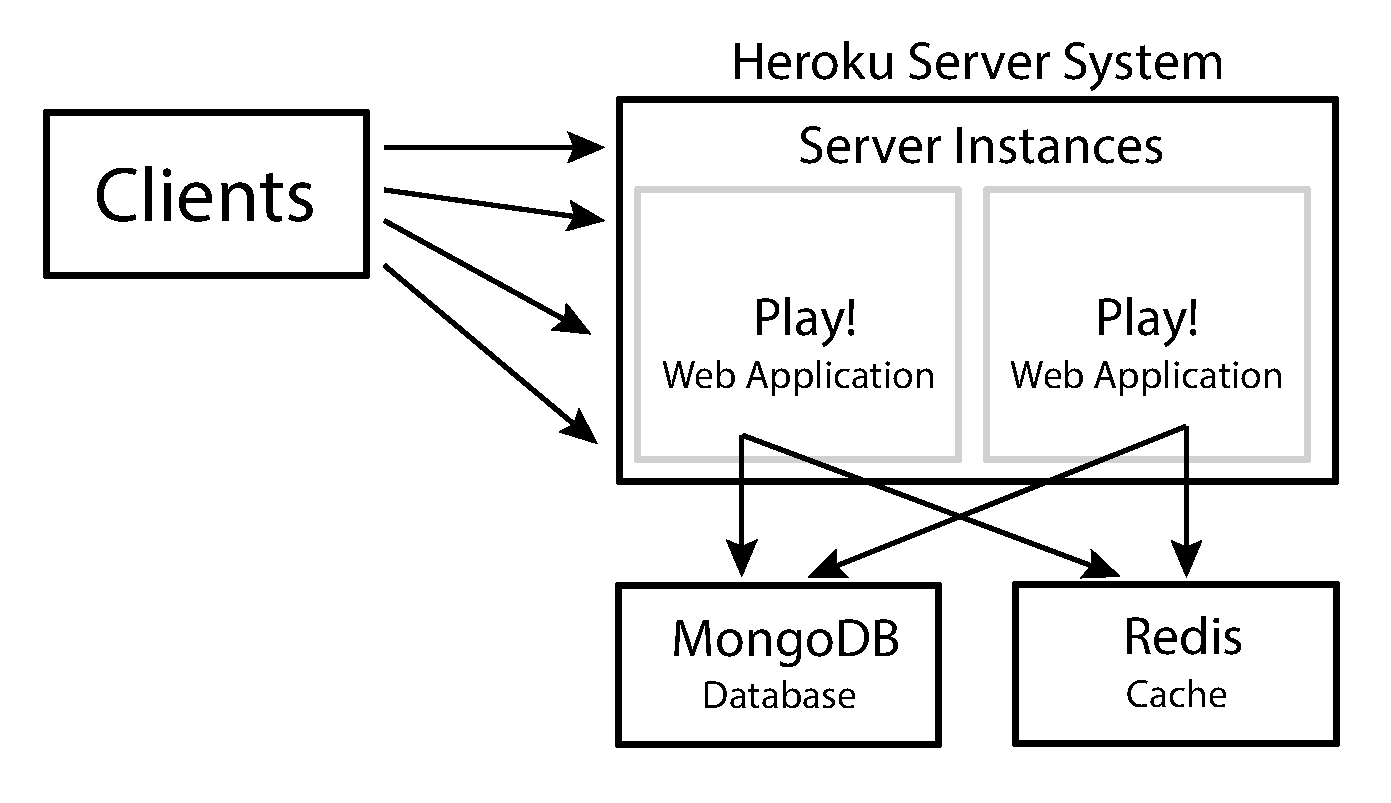
\includegraphics[width=.80\textwidth]{project}
\caption{
The final project setup that resulted from the preceding considerations. Note that client requests are distributed among server instances by the server system, but every server instance connects to the database and cache individually.
}
\label{fig:project}
\end{figure}

The application also makes use of several other libraries, e.g. for sending emails. Here, a great advantage of \textit{Scala} comes 
into play: due to being compiled to \textit{Java} bytecode, \textit{Scala} is binary compatible with all available \textit{Java} libraries. For instance, the \textit{Apache Commons}\footnote{\url{http://commons.apache.org/}} email implementation written in \textit{Java} can also be used to send emails in \textit{Scala}\footnote{Blocking \textit{Java} functions can also be wrapped with \textit{Futures} (see sections \ref{lab:play} and \ref{lab:basicasync}) in order to create non-blocking, actor-based \textit{Scala} functions.}.

\section{Development}
\label{lab:impl-dev}

This section describes how actor-driven patterns were used to realise relevant parts of a Web server application with respect to the prerequisites defined in the last section.

\subsection{Requests and Actions}
As already mentioned in section \ref{lab:play}, \textit{Play!} uses different controller actions to determine if a request should be served synchronously or asynchronously (see program \ref{prog:scala-actions1} and \ref{prog:scala-actions2}, respectively). A good example for a synchronous request is an action that returns the current server time for the request signing procedure\footnote{Requests are only valid for a certain timespan to prevent \textit{replay attacks}, i.e. capturing and sending a request multiple times.}. Here, no database action is necessary and the retrieval of system time does not consume much processing time. However, nearly all requests to the Web server involve some kind of database operation; either resources are read or written or a combination of multiple operations is executed. When writing a value to the database, the response is served after the operation completes to indicate success or failure to the client; this way, the client can decide for itself whether it waits for the response or, for instance, updates the user interface right after sending the request.

\subsection{Basic Asynchronous Operations}
\label{lab:basicasync}



\subsubsection*{Working With Futures}
The majority of asynchronous operations involve database or cache access. The database driver and the cache driver both return \texttt{Future} objects, i.e. the respective calls return almost instantaneously and yield a value that is resolved later (cf. program \ref{prog:scala-actions2}). In the simplest case, this value can be mapped to a \texttt{Result} object and returned by an asynchronous action. However, this is not always the case; frequently, the returned value has to be processed and results are even used as parameters for new database operations. Program \ref{prog:multimap} shows an example with two nested \texttt{Future} resolutions.

A typical occurrence of two database operations is for instance when a new user should be created with a unique username. The outmost block is the default asynchronous \texttt{Action} block with a \textit{body parser} as argument. This body parser converts the text from the request body into a JSON  object\footnote{JavaScript Object Notation, commonly used for HTTP communication, \url{http://json.org/}} suitable for further processing. This body must contain a desired username, which is obtained by traversing the JSON abstract syntax tree (using the \textbackslash{} method). Next, a database query is initiated using the provided username. This query returns a \texttt{Future[Option[User]]} object; the \texttt{Option} type indicates that the value can either be present (\texttt{Some}) or absent (\texttt{None}). The \texttt{flatMap} method is similar to the \texttt{map} method, but instead of \texttt{Result} objects, all statements inside the block must return \texttt{Future[Result]} objects. If the database query returns an object of the type \texttt{None}, no user with the given username is found and thus the new user can be inserted and the result of the database operation can be mapped to a \texttt{Result} using \texttt{map}. However, if the username already exists, no subsequent database operation has to be initiated and the response can be sent instantly. To generate a readily resolved \texttt{Future}, the \texttt{Future.successful} method can be used.

\begin{program}
  \caption{This is a basic example of how two database operations can be nested in a \textit{Play!} application. \texttt{Created}, \texttt{Conflict} and \texttt{InternalServerError} are helpers for the response status codes \texttt{201}, \texttt{409} and \texttt{500}, respectively.}
  \label{prog:multimap}
  \begin{JavaCode}
def insertUniqueUser() = Action.async(parse.json) {
    request =>
        val username = (request.body \ "username").as[String]
        UserService.findByUsername(username) flatMap {
            case None =>
                UserService.insert(request.body) map {
                    case Some(id) =>
                        Created("New user created with id " + id)
                    case None =>
                        InternalServerError("User could not be created")
                }
             case Some(user) =>
                Future.successful(Conflict("Username exists!"))
        }
}
  \end{JavaCode}
\end{program}

\begin{program}
  \caption{In this example, two images are uploaded to a remote server. Only when both uploads have completed, the response should be sent containing the URLs oft both images. The \texttt{for} comprehension receives a block with multiple \texttt{Future[String]} assignments. The \texttt{yield} statement wraps these \texttt{Future} objects in a single \texttt{Future[(String, String)]} object. This is a type called a \textit{tuple}, i.e. two objects combined into one. The \texttt{map} comprehension in line 4 maps this \texttt{Future} to a simple tuple, the values of which can be retrieved using the \texttt{.\_1} and \texttt{\_.2} properties (line 6).}
  \label{prog:for}
\begin{JavaCode}
(for {
    picture1Url <- uploadPicture(picture1)
    picture2Url <- uploadPicture(picture2)
} yield (picture1Url, picture2Url)) map {
    result =>
        Ok("Here are your pictures:\n" + result._1 + "\n" + result._2)
}
\end{JavaCode}
\end{program}

To resolve multiple \texttt{Future} objects in parallel and work with the combined results of the single asynchronous operations, the \texttt{for} comprehension can be used; see program \ref{prog:for} for an example.

Apart from database and cache operations, \texttt{Future} objects also result from using \textit{Play!}'s integrated \texttt{WS} Web service library. Since HTTP requests take an arbitrary amount of time to return, the use of asynchronous processing yields high performance gains since this way, a potentially slow third-party Web server only delays the application's response to the client, but does not inflict the application's performance by blocking threads. 

\subsubsection*{Deferring Program Flow}
Certain operations are not relevant to the further program flow and can be executed concurrently without the need for resolving return values. These \textit{asynchronous side-effects} can be executed at any point during program flow. For instance, if the user requests that his photo album should be deleted, the request may return as soon as the album object is removed from the database, but the deletion of the actual image files (which may take some time) can be deferred to a later point in time:

\begin{JavaCode}
def deleteAlbum(id: String) = Action.async {
    AlbumService.deleteById(id) map {
        case true =>
            ImageService.deleteForAlbum(id)
            Ok("Your album was deleted!")
        case false =>
            InternalServerError("Something went wrong!")
    }
}
 
\end{JavaCode}

Deferring execution can also be done using \textit{Akka}'s scheduling functionality. The present application uses this scheduling functionality to obtain a new \textit{access token} for authentication from Web services, depending on when the old token expires. The execution can be scheduled at a specific point in time or repeated periodically:
\begin{JavaCode}
import play.api.libs.concurrent.Akka

Akka.system.scheduleOnce(10.minutes)(sendReminderEmail())

// The first parameter defines the initial delay, the second one the interval
Akka.system.schedule(Duration.Zero, 30.minutes)(renewAccessToken())

\end{JavaCode}

Technically, actors can also be used to defer program flow, but are generally used for more sophisticated operations (see section \ref{lab:explicit-actors}).

\subsubsection*{Converting Blocking Code}
Of course, not all operations return asynchronous results, especially when using third-party or \textit{Java} libraries. Wrapping blocking method calls in \texttt{Future} objects that can be resolved by \textit{Akka} is rather trivial:
\begin{JavaCode}
def asynchronousOperation(param: String): Future[String] = {
    Future {
        synchronousOperation(param)
    }
}
\end{JavaCode}

When resolving \texttt{Future} objects within a \textit{Play!} application, \textit{Play!}'s default dispatcher is used (for information about dispatchers see section \ref{lab:play}, \textit{Scalability}). However, especially for computationally expensive operations like image processing it is advisory to use a dedicated dispatcher. New dispatchers can be created by defining them in the \textit{Akka} configuration within \textit{Play!}'s configuration files (see program \ref{prog:customdispatcher}).
\begin{program}
  \caption{This configuration statement defines a custom dispatcher called \texttt{image-processing-dispatcher} that uses a \textit{fork-join executor} and at most two threads in order not to block the application.}
  \label{prog:customdispatcher}
\begin{JavaCode}
akka {
    actor {
        image-processing-dispatcher {
            fork-join-executor {
                parallelism-max = 2
            }
        }
    }
}
\end{JavaCode}
\end{program}
Program \ref{prog:convert} gives an example of an expensive image processing operation converted to an asynchronous operation that can be deferred using a custom dispatcher. At the beginning of the code example, a reference to the custom dispatcher is created using \textit{Akka}'s lookup functionality. The \texttt{Future} block wraps the expensive operation and defines the dispatcher that should be used to resolve the \texttt{Future} object (i.e. how it should be processed by the actor system). The operation itself consists of a operating system call to a image processing command line tool. The \texttt{waitFor} method blocks the dedicated dispatcher thread until the processing has finished. After that, the \texttt{Future} object is resolved with a \texttt{File} reference to the generated image.

\begin{program}
  \caption{This program shows how a comparably expensive image processing operation can be deferred using a custom dispatcher.}
  \label{prog:convert}
  \begin{JavaCode}
val dispatcher = Akka.system.dispatchers.lookup("akka.actor.image-processing-dispatcher")

def generateImage(filename: String): Future[File] = {

    Future {

        val cmd = Array(
            "convert",
            "-background", "black",
            "-fill", "white",
            ...
            filename
        )

        Runtime.getRuntime.exec(cmd).waitFor()

        new File(filename)
    
    } (dispatcher)
    
}
  \end{JavaCode}
\end{program}


\subsection{Actor-based Operations}
\label{lab:explicit-actors}
Since \textit{Play!} does not expose the underlying actor structure to its libraries, application can be built without explicitly using any actors. However, the present application uses four actors for complex concurrency operations: the \texttt{Mailman} and \texttt{Notifier} actors are used to defer and isolate complex asynchronous operations, namely sending emails and mobile notifications, respectively. These two actors are structurally rather similar to the \texttt{Mailer} actor presented in program \ref{prog:scala-actors}, but include extensive logic to generate the different notifications depending on the received actor message. However, the \texttt{Feeder} and \texttt{Subscriber} actors are more complex and play an important role in section \ref{lab:news}.

\subsection{Advanced Actor Usage}
\label{lab:news}
The application also includes a news feed using a technology called \textit{Websockets} to send events to subscribed client applications over TCP. The basic idea is that when one user takes a specific action, other users that are interested in that action get notified instantly. A rather trivial approach would be to keep a collection of currently subscribed clients and notify them directly when a certain event occurs according to what events they have subscribed to. However, as defined in section \ref{sec:prerequitites}, \textit{Requirements}, the application should be scalable to multiple systems. This introduces a problem: clients that subscribed on one particular system will not get events that occurred on other systems since the event is not propagated across all systems.

The solution is to use a centralised messaging system. Options include dedicated protocols like \textit{AMQP}\footnote{Asynchronous Message Queuing Protocol, \url{http://www.amqp.org/}}, but since the application already uses \textit{Redis}, which supports the \textit{Pub/Sub}\footnote{Publish-Subscribe, for \textit{Redis} implementation see \url{http://redis.io/topics/pubsub}} paradigm, using this system is more practicable. \textit{Pub/Sub} works by publishing messages to the central server, which forwards them to all systems who have subscribed to the corresponding message type.

Publishing to the \textit{Redis} server can be easily done using the \textit{rediscala} library; for instance, the following line of code is used to publish a message when a user \texttt{abcd} likes a photo \texttt{1234}:
\begin{JavaCode}
RedisService.publish("/picture/1234/likes", "abcd")
\end{JavaCode}
Due to the side-effect nature of publishing a message, this may also be done using an actor. 

Subscribing and receiving messages is the more complex part of the centralised message passing lifecycle. Ideally, incoming \textit{Redis} messages should be translated to \textit{Akka} messages for subsequent handling inside the actor system. Fortunately, \textit{rediscala} includes the \texttt{RedisSubscriberActor} superclass to facilitate subscribing to messages. Program \ref{prog:subscriber} shows how this subscriber actor class is structured and used to receive custom \textit{Redis} \texttt{publish} messages. Besides the publish channel, \textit{Redis} messages may include a pattern signature; messages are then only distributed to the subscribers that signify interest in the particular pattern. To be able to use the \texttt{RedisSubscriberActor} superclass, the subscriber actor has to supply two methods. The \texttt{onMessage} method is called when a message without a pattern arrives; however, because in this case only pattern messages are used, this message can return an empty object. The \texttt{onPMessage} method receives pattern messages and \textit{tells} the \texttt{Feeder} actor to send the message to the currently connected clients. The subscriber actor has to be initialised upon application start; this can be done using \textit{Play!}'s \texttt{Global} object, which can override the \texttt{onStart} method. Inside the \texttt{onStart} method, the subscriber actor is created using the \texttt{Props} object, which creates a new class instance using specified constructor parameters. The second parameter, \texttt{Nil}, indicates, that the subscriber should not listen to a particular channel; the third parameter is a sequence of patterns consisting of one pattern that matches likes for any picture. Note that this actor uses \textit{rediscala}'s own dispatcher. A diagram of how information flow happens within the setup can be seen in figure \ref{fig:subscribe}.

\begin{program}
  \caption{This program shows how the \texttt{RedisSubscriberActor} superclass can be used to create an actor class that listens for custom \textit{Redis} \texttt{publish} messages.}
  \label{prog:subscriber}
  \begin{JavaCode}
class Subscriber(channels: Seq[String] = Nil, patterns: Seq[String] = Nil) extends RedisSubscriberActor(Redis.socket, channels, patterns, Redis.password) { 
 
    def onMessage(message: Message) {
        Nil
    }

    def onPMessage(message: PMessage) {
        Feeder.push((message.channel, message.data))
    }

}

object Global {

    override def onStart(app: Application) = { 
        Akka.system.actorOf(Props(classOf[Subscriber], Nil, Seq("/picture/*/likes")).withDispatcher("rediscala.rediscala-client-worker-dispatcher"))
    }

}
  \end{JavaCode}
\end{program}

\begin{figure}
\centering\small
\setlength{\tabcolsep}{0mm}
  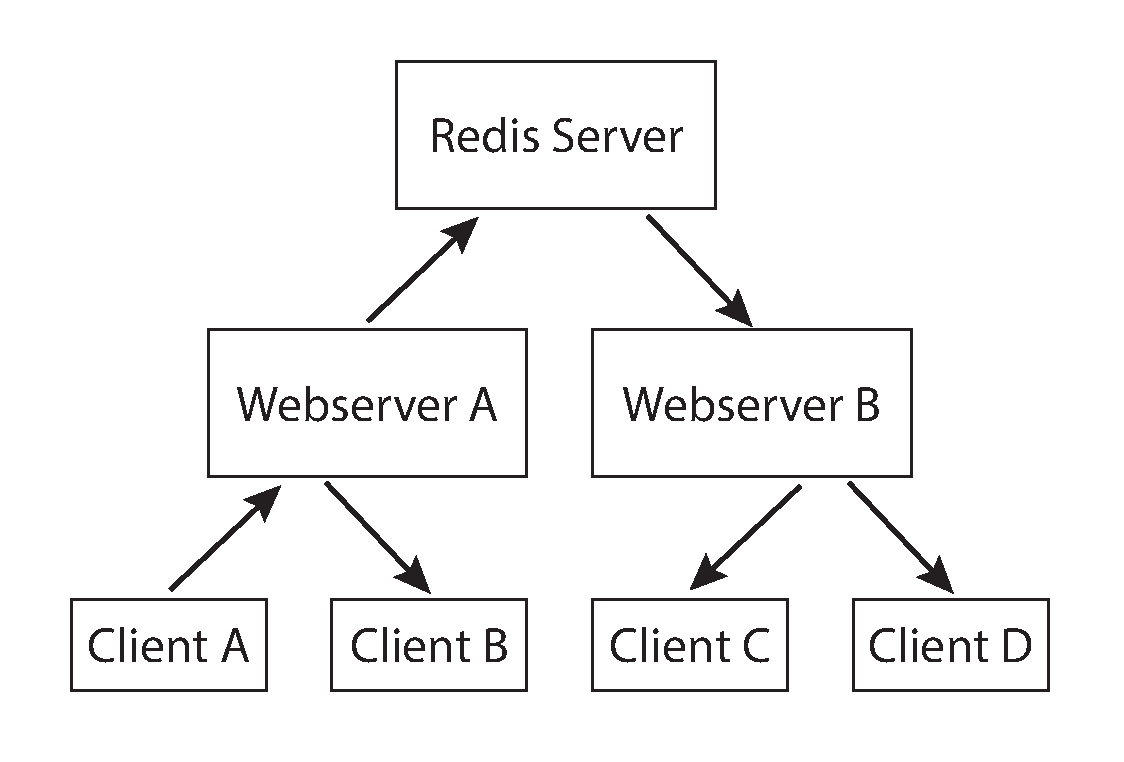
\includegraphics[width=.80\textwidth]{subscribe}
\caption{
Schematic information flow between systems and clients. Client A triggers an event, e.g. likes a picture, which concerns the other three clients. The event is processed by server A, which sends the information directly to all connected clients. Server A \textit{publishes} the event also to the central \textit{Redis} server, which propagates it to all subscribed servers. Server B then sends the received information on to all connected clients.
}
\label{fig:subscribe}
\end{figure}


The fourth and last actor, is the \texttt{Feeder} actor. This is a standard actor that listens for two types of messages: 
\begin{itemize}
  \item{If a client connects to the application via \textit{Play!}'s \texttt{WebSocket.tryAccept} controller action, the actor receives a message containing the desired feed (e.g. \texttt{/picture/1234/likes}) and a reference handle to the client. The actor then stores the client inside a collection.}
  \item{If a feed message arrives, the actor iterates over its client collection and identifies clients that have indicated interest in the message. The actor then sends relevant information (like which user has liked which picture) to the client over the \textit{WebSocket}.}
\end{itemize}

\section{Deployment and Scaling}
The described \textit{Play!} application can run on any platform that can execute \textit{Java} bytecode. Since it even includes its own Web server, it represents an integrated container that is readily suitable for deployment over multiple server instances. The present application is designed to use identical replications of actor systems on every system, the only means of sharing application state being the message passing via the \textit{Redis} server (see program \ref{prog:subscriber}). This means that the application can theoretically be scaled out indefinitely, provided a \textit{load balancer} serves incoming requests fast enough to the server instances and the database and cache communication happens at a formidable speed.

A \textit{Play!} application could be scaled out in a different way: instead of automated replications, the application could be designed using different modules on different systems that communicate via a central \textit{Akka} system. This way, a number of systems could handle network I/O and other systems could handle side effects or intensive computations like image processing.
